\documentclass[12pt, letterpaper]{article}

\usepackage[utf8]{inputenc}
\usepackage[framemethod=TikZ]{mdframed}
\usepackage[hidelinks]{hyperref}
\usepackage{mathtools, amssymb, amsmath, cleveref, fancyhdr, geometry, tcolorbox, graphicx, float, subfigure, arydshln, url, setspace, framed, pifont, physics, ntheorem, utopia}
%%% for coding %%%
\usepackage{listings}
\usepackage[ruled, vlined, linesnumbered]{algorithm2e}

\geometry{letterpaper, left=2cm, right=2cm, bottom=2cm, top=2cm}

\pagestyle{fancy}
\fancyhead{}
\fancyhead[L]{\leftmark}
\fancyhead[R]{\rightmark}
\fancyfoot{}
\fancyfoot[C]{\thepage}
%\renewcommand{\headrulewidth}{0pt}
\renewcommand{\footrulewidth}{0pt}

\hypersetup{
	colorlinks = true,
	bookmarks = true,
	bookmarksnumbered = true,
	pdfborder = 001,
	linkcolor = blue
}

\definecolor{emoryblue}{RGB}{1, 33, 105} 
\definecolor{lightblue}{RGB}{0, 125, 186}
\definecolor{mediumblue}{RGB}{ 0, 51, 160}
\definecolor{darkblue}{RGB}{12, 35, 64}
\definecolor{red}{RGB}{185, 58, 38}
\definecolor{green}{RGB}{72, 127, 132}
\definecolor{gray1}{RGB}{217, 217, 214}
\definecolor{gray5}{RGB}{177, 179, 179}
\definecolor{gray3}{RGB}{208, 208, 206}

\definecolor{grey}{rgb}{0.49,0.38,0.29}
\definecolor{mygreen}{rgb}{0,0.6,0}
\definecolor{grey}{rgb}{0.49,0.38,0.29}
\definecolor{mygreen}{rgb}{0,0.6,0}


%%% for coding %%%
\lstset{basicstyle = \ttfamily\small,commentstyle = \color{mygreen}\textit, deletekeywords = {...}, escapeinside = {\%*}{*)}, frame = single, framesep = 0.5em, keywordstyle = \bfseries\color{blue}, morekeywords = {*}, emph = {self}, emphstyle=\bfseries\color{red}, numbers = left, numbersep = 1.5em, numberstyle = \ttfamily\small\color{grey},  rulecolor = \color{black}, showstringspaces = false, stringstyle = \ttfamily\color{purple}, tabsize = 4, columns = flexible}


\newcounter{index}[subsection]
\setcounter{index}{0}
\newenvironment*{df}[1]{\par\noindent\textbf{Definition \thesubsection.\stepcounter{index}\theindex\ (#1).}}{\par}

\newenvironment*{eg}[1]{\begin{framed}\par\noindent\textbf{Example \thesubsection.\stepcounter{index}\theindex\ #1}\par }{\par\end{framed}}

\newenvironment*{thm}[1]{\begin{tcolorbox}[colback=lightblue!5,colframe=darkblue!90, title=\textit{\textbf{Theorem \thesubsection.\stepcounter{index}\theindex}\ {#1}}]}{\par\end{tcolorbox}}

\newenvironment*{clm}{\begin{tcolorbox}[colback=mygreen!10, colframe=green, title=\textit{\textbf{Claim \thesubsection.\stepcounter{index}\theindex}}]}{\par\end{tcolorbox}}

\newenvironment*{cor}[1]{\par\noindent\textbf{Corollary \thesection.\stepcounter{index}\theindex\ #1:}}{\par}
\newenvironment*{lem}[1]{\par\noindent\textbf{Lemma \thesection.\stepcounter{index}\theindex\ #1:}}{\par}
\newenvironment*{ax}[1]{\par\noindent\textbf{Axiom \thesection.\stepcounter{index}\theindex\ #1:}}{\par}
\newenvironment*{prop}[1]{\par\noindent\textbf{Proposition \thesection.\stepcounter{index}\theindex\ #1:}}{\par}
\newenvironment*{conj}[1]{\par\noindent\textbf{Conjecture \thesection.\stepcounter{index}\theindex\ #1:}}{\par}
\newenvironment*{nota}{\par\noindent\textbf{Notation \thesection.\stepcounter{index}\theindex.}}{\par}

\newcounter{nprf}[subsection]
\setcounter{nprf}{0}
\newenvironment*{prf}{\par\indent\textbf{\textit{Proof \stepcounter{nprf}\thenprf.}}}{\hfill$\blacksquare$\par}
\newenvironment*{dis}{\par\indent\textbf{\textit{Disproof \stepcounter{nprf}\thenprf.}}}{\hfill$\blacksquare$\par}
\newenvironment*{sol}{\par\indent\textbf{\textit{Solution \stepcounter{nprf}\thenprf.}}\par}{\hfill{$\square$}\par}

\newenvironment*{prf*}{\par\indent\textit{Proof.}\ }{$\qquad\square$\par}
\newenvironment*{dis*}{\par\indent\textit{Disproof.}\ }{$\qquad\square$\par}
\newenvironment*{sol*}{\par\indent\textit{Solution.}\ }{$\qquad\square$\par}

\newtheorem{hint}{Hint}[section]
\newtheorem{rmk}{Remark}[section]
\newtheorem{ext}{Extension}[section]

\newtheorem*{df*}{Definition}
\newtheorem*{thm*}{Theorem}
\newtheorem*{clm*}{Claim}
\newtheorem*{cor*}{Corollary}
\newtheorem*{lem*}{Lemma}
\newtheorem*{ax*}{Axiom}
\newtheorem*{prop*}{Proposition}
\newtheorem*{conj*}{Conjecture}
\newtheorem*{nota*}{Notation}

\linespread{1.25}

\newcommand{\inprod}[2]{\left\langle #1, #2 \right\rangle}
\def\Z{{\mathbb{Z}}}
\def\R{{\mathbb{R}}}
\def\C{{\mathbb{C}}}
\def\Q{{\mathbb{Q}}}
\def\E{{\mathbb{E}}}
\def\d{{\mathrm{d}}}
\def\i{{\mathrm{i}}}

\newcommand{\inprod}[2]{\left\langle #1, #2 \right\rangle}
\def\Z{\mathbb{Z}}
\def\R{\mathbb{R}}
\def\C{\mathbb{C}}
\def\Q{\mathbb{Q}}
\def\N{\mathbb{N}}
\def\d{\mathrm{d}}
\def\1{\mathds{1}}
\def\epsilon{\varepsilon}
\def\emptyset{\varnothing}
\def\phi{\varphi}
\def\dsst{\displaystyle}
\def\st{\ s.t.\ }
\def\bar{\overline}
\def\E{\vb{E}}
\def\B{\vb{B}}
\def\L{\vb{L}}
\def\I{\vb{I}}
\def\Var{\vb{Var}}
\def\V{\vb{Var}}
\def\Cov{\vb{Cov}}
\def\MSE{\vb{MSE}}
\def\P{\vb{P}}
\def\M{\vb{M}}
\def\iid{i.i.d.}
\def\argmax{\arg\max}
\def\argmin{\arg\min}
\def\l{\ell}
\def\hat{\widehat}
\def\independ{\perp\!\!\!\perp}
\def\depend{\leftrightsquigarrow}
\def\residual{\varepsilon}
\def\sd{\mathrm{sd}}

\title{Emory University\\\textbf{QTM 220 Regression Analysis}\\ Learning Notes}
\author{Jiuru Lyu}
\date{\today}

\begin{document}
\maketitle

\tableofcontents

\newpage
\section{Statistical Inference}
\subsection{Descriptive Statistics and Binary Covariates}
\begin{df}{Location}
	The \textit{location} of the data is where it is. It is about approximating the data by a constant. \[Y_i\approx\mu,\quad\text{for }i=1,\dots,n\]	
\end{df}
\begin{eg}
	Different ways to summarize location: mean, median
\end{eg}
\begin{df}{Spread}
	The \textit{spread} of the data is how far it tends to be from is location. 	
\end{df}
\begin{df}{Residuals}
	Spread summarizes the size of the \textit{residuals} left over after constant approximation. We use $\hat\epsilon$ to denote residuals. \[\residual_i\coloneqq Y_i-\hat\mu.\]
\end{df}
\begin{df}{Median Absolute Deviation and Standard Deviation}
	\begin{itemize}
		\item The \textit{median absolute deviation (MAD)} is the median size of residuals.
		\item The \textit{standard deviation (sd)} is the square root of the mean squared size of residuals. 
		\begin{rmk}The standard deviation is a sort of average in which big residuals count more than smaller ones. \end{rmk}
	\end{itemize}
\end{df}
\begin{df}{Distribution}
	We use \textit{histograms} to summarize the \textit{distribution} of the data. 
\end{df}
\begin{rmk}
	Distribution of the data tells us more information than location and spread, but less than dot plot. \emph{For example, in this context, dot plot also include the identities of the individuals in addition to the number of people having salary in the range. }
\end{rmk}
\begin{df}{Binary Data}
	\textit{Binary data} only have two options, and we usually denote those two options as $1$'s and $0$'s. 	
\end{df}
\begin{cor}{}
	Hence, when drawing a dot plot, everyone falls into either of the two lines representing $1$ and $0$.
\end{cor}
\begin{thm}{Location of Binary Data}
	The median is whichever outcome is the most common, and the mean is the proportion of $1$'s in the data. 
\end{thm}
\begin{rmk}
	Hence, a histogram tells us no more information than $\hat\mu$.	
\end{rmk}
\begin{thm}{Spread of Binary Data}
	\begin{itemize}
		\item Median absolute deviation will always be $0$ in a binary case.
		\item The standard deviation is the square root of the mean squared distance from the mean, and \[\text{sd}=\sqrt{\hat\mu\qty(1-\hat\mu)}.\]
	\end{itemize}
\end{thm}
\begin{prf}
	The claim concerning MAD is trivial. \textit{Hint: there's only two possible values in the data, so median and MAD should always be the same.}\par Now, let's consider the claim on standard deviation. \begin{align*}\sd^2&=\dfrac{1}{n}\sum_{i=1}^n\qty(Y_i-\hat\mu)^2\\&=\dfrac{1}{n}\sum_{y:\qty{0,1}}\sum_{i:Y_i=y}\qty(Y_i-\hat\mu)^2\\&=\dfrac{1}{n}\qty{N_1\qty(1-\hat\mu^2)+\qty(n-N_1)\qty(0-\hat\mu^2)}&[N_1=\text{number of }1\text{'s}]\\&=\dfrac{1}{n}\qty{N_1\qty(1-2\hat\mu+\hat\mu^2)+\qty(n-N_1)\hat\mu^2}\\&=\dfrac{1}{n}\qty{N_1-2N_1\hat\mu+n\hat\mu^2}\\&=\dfrac{1}{n}\qty{n\hat\mu-2n\hat\mu\cdot\hat\mu+n\hat\mu^2}&[N_1=n\hat\mu]\\&=\dfrac{1}{n}\qty{n\hat\mu-n\hat\mu^2}\\&=\hat\mu-\hat\mu^2=\hat\mu\qty(1-\hat\mu).\end{align*} Therefore, we know \[\sd=\sqrt{\hat\mu\qty(1-\hat\mu)}.\]
\end{prf}
\begin{rmk}
	In binary data, knowing the mean $\equiv$ knowing everything else. 
\end{rmk}

\subsection{Population Inference for a Proportion}
\begin{df}{Sampling Distribution}
	The \textit{sampling distribution} is the distribution of estimates we'd get if we \textbf{replicated} our experiment over and over. 
\end{df}
\begin{itemize}
	\item Think of lots of people rolling the dice and reporting what they got. 
	\item We consider this because it actually tells us something: it gives us an \textbf{interval} we can expect the proportion is in, and a statement about how much \textbf{confidence} we should have about it. 
\end{itemize}
\begin{eg}{Connecting Sample and Population}
	For each call $i$, we randomly select a voter with an id we'll call $J_i$. And we record as the call's outcome the turnout of the voter: $Y_i=y_{J_i}$. We can run this simulation using \texttt{R}. 
	\begin{center}
		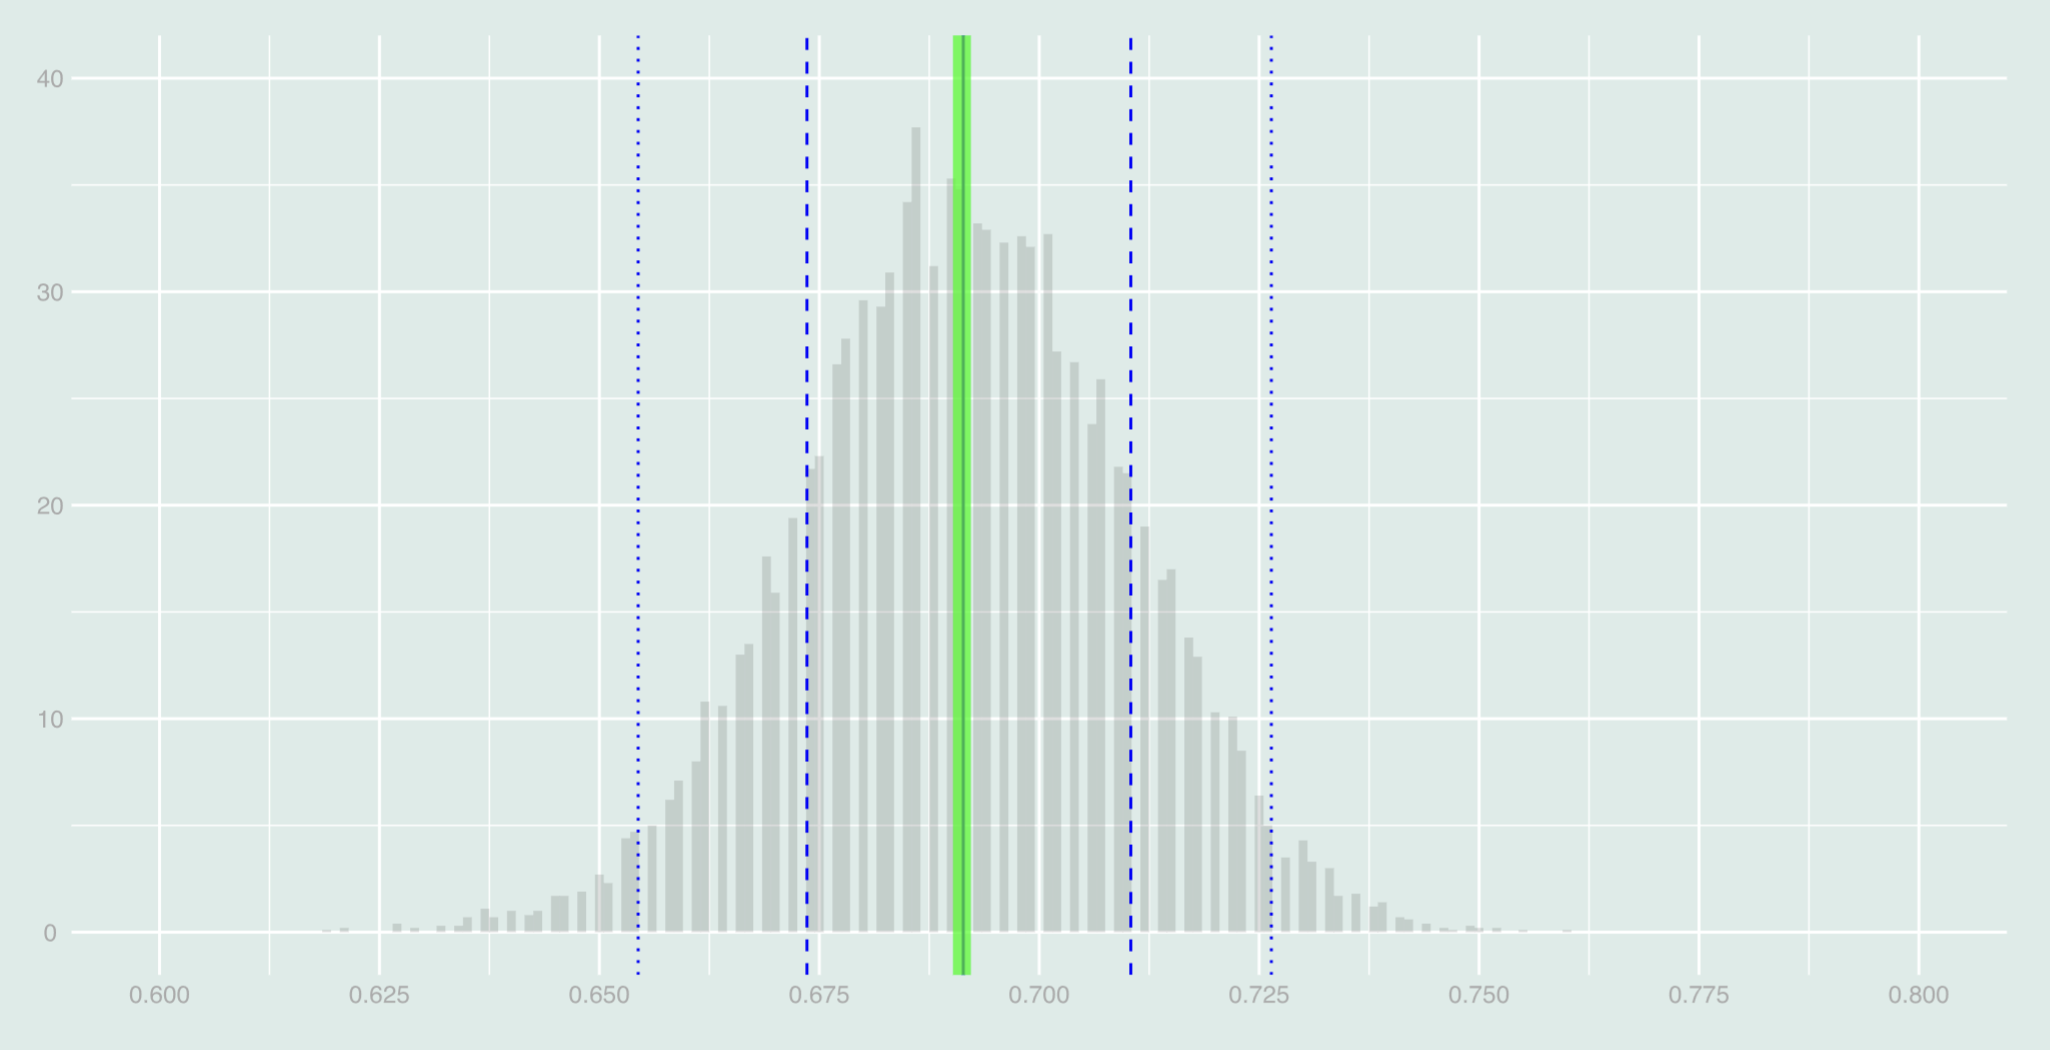
\includegraphics[width=0.7\textwidth]{figs/SamplingDistribution.png}	
	\end{center}
	\begin{itemize}
		\item The \textit{mean of the sampling distribution} is the solid blue line.
		\item The middle 2/3 of the sampling distribution lies between the dashed blue lines.
		\item The middle 95\% of the sampling distribution lies between the dotted blue lines. 
		\item Also, the population proportion is drawn as a wide green line. 
		\item The question is ``Could we predict how close we can get from the sampling before the election happened?'' -- Yes!
		\begin{itemize}
			\item We will use an \textbf{interval estimate}: a \textit{range of values} the population proportion is likely to be in.
			\item The \textbf{width} of this interval speaks to the ``how close'' question.
			\item The \textbf{coverage probability} (the probability we are right) qualifies this answer.
			\begin{itemize}
				\item Our \textbf{point estimate} of the population proportion is the sample proportion $\bar{Y_n}$, where $n$ is the size of the sample. 
				\item Now, we will try with some size of the interval. Say, $x$. Then, we are interested in the range of data $\bar{Y_n}\pm\dfrac{x}{2}$ (since the interval can be two-tailed).
				\item Repeat the sampling process multiple times, say $M$ times, and we notice that out of $t$ times our interval ``touches'' the population proportion. 
				\item Then, we can define the coverage probability as follows: \[\text{coverage probability}=\dfrac{t}{M}=\P\qty(\bar{Y}_n\in\bar{y}_N\pm \dfrac{x}{2}),\] where $\bar{Y}_n$ is our point estimate, $\bar{y}_N$ is the population proportion, and $x$ is the width of the interval. 
			\end{itemize} 
		\end{itemize}
		\item Most of the time, we would like a 95\% coverage probability, which means we will need to use a wider interval. 
		\item Therefore, what we want to do is to choose a coverage probability and calculate the right width. An interval estimate like this (to ensure a given coverage) is called a \textbf{confidence interval}.
		\item The following figure shows a 95\% coverage probability: \begin{center}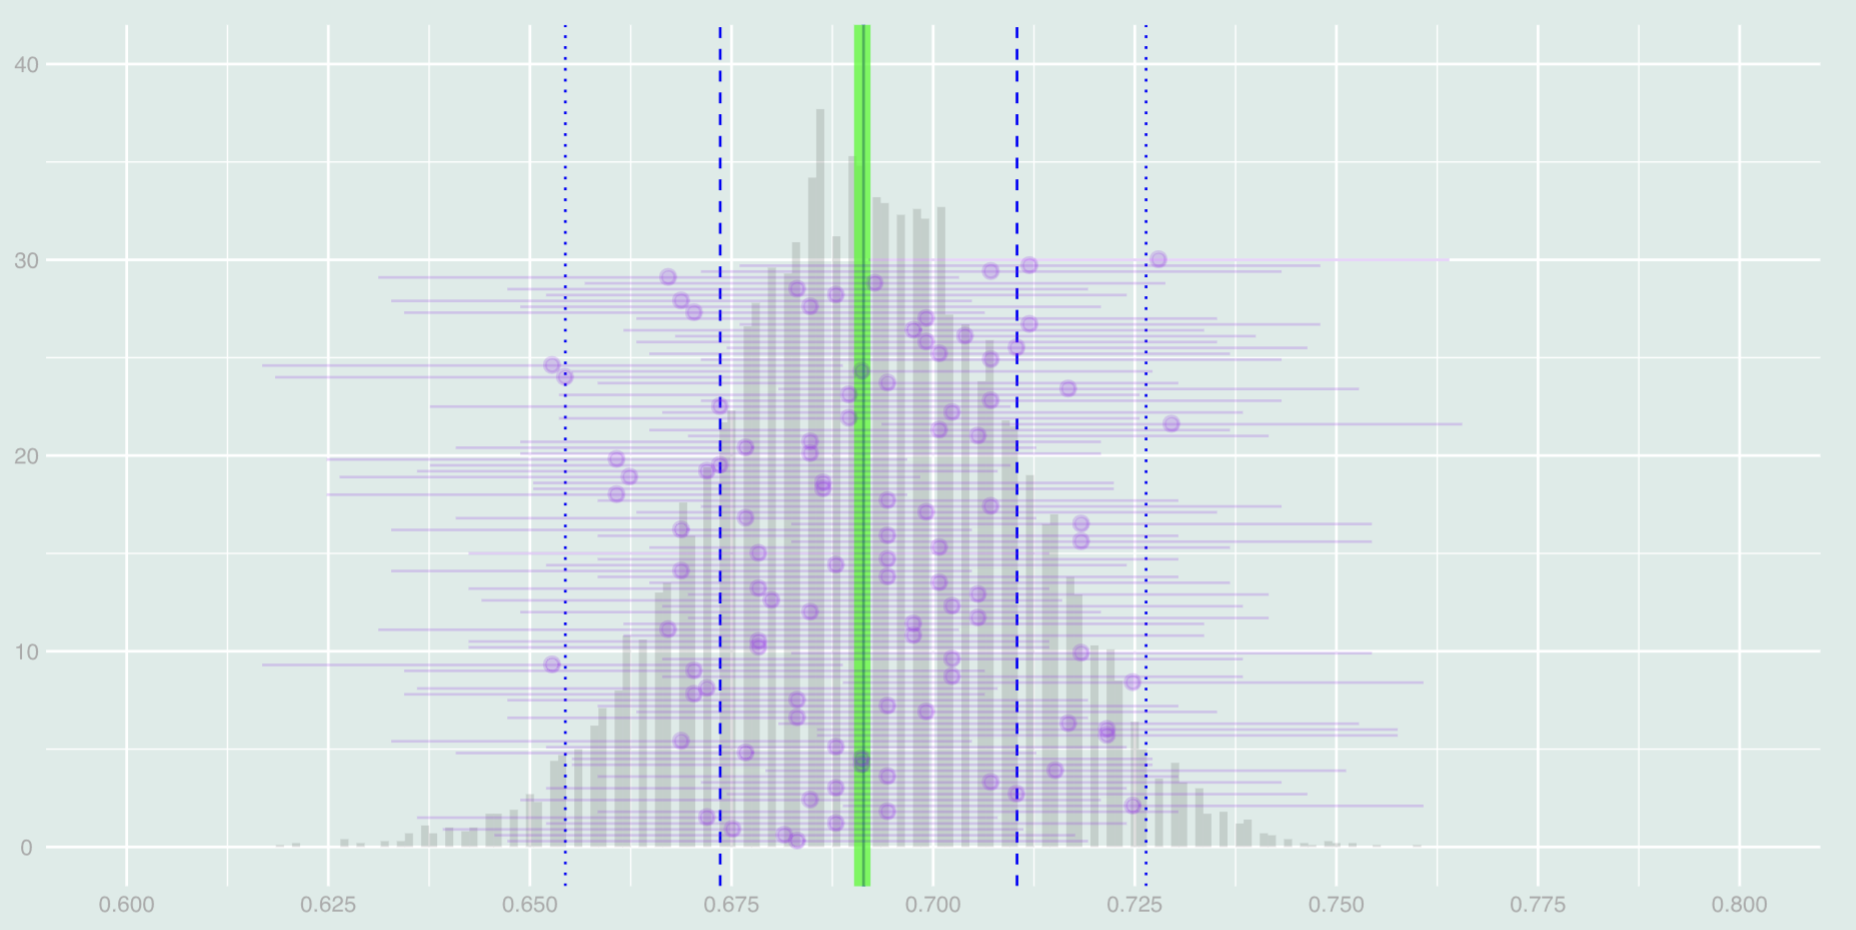
\includegraphics[width=0.7\textwidth]{figs/95ConfidenceInterval.png}\end{center}
		\begin{itemize}
			\item Our sample proportion $0.68$ is close to the population proportion $0.69$. Did we get luck? \textit{No! In a million runs, almost all are within 0.05}.
			\item Could we have predicted how close we would get before seeing the $0.69$? \textit{Yes! We can use a calibrated interval estimate -- a Confidence Interval}.
		\end{itemize}
		\item However, notice that this approach is not perfect: we cannot calibrate intervals like this in real life. 
		\begin{itemize}
			\item When we run our pool, we get a single point estimate $\bar{Y}_n$ based on our sample. 
			\item We don't know the sampling distribution of this point estimate until the election day.
			\item However, what we actually do is almost the same: we will use an estimate of the sampling distribution in place of the thing itself. 
		\end{itemize} 
	\end{itemize}
\end{eg}

\subsection{Calibrating Interval Estimates}
\begin{thm}{}
	An interval estimate covers the population proportion $\iff$ the corresponding point estimate is between the population proportion's arms.	
\end{thm}

\begin{rmk}
	With this Theorem, in Example 1.2.2, instead of looking at every interval and its arms to calculate coverage, we can draw arms of the same width around the population proportion. \par Equivalently, we can calculate the \textbf{mass of the histogram} between the population proportion's arms. \par However, even with this Theorem, the problem still exists: unless we've seen the population, we cannot run simulations. Hence, in reality we will do calibration using an \textbf{estimate of the sampling distribution}.
\end{rmk}
\begin{eg}{}
	Here, we use our sample to estimate the sampling distribution. Compared with the actual population mean, the sample mean is a bit lower. Will this impact our estimation?
	\begin{center}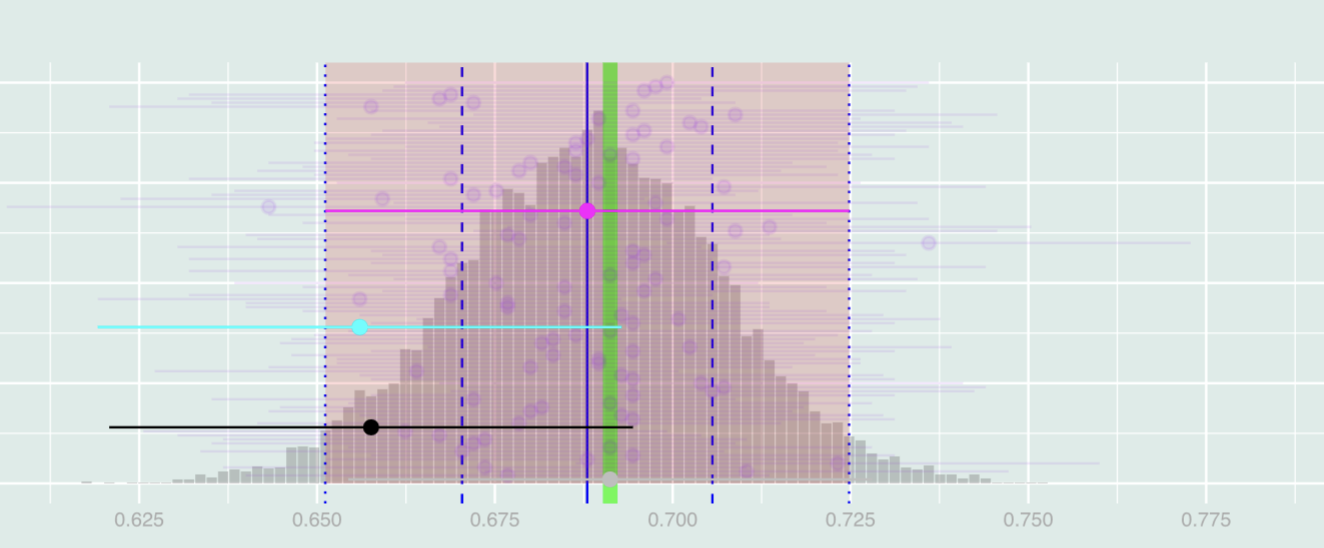
\includegraphics[width=0.7\textwidth]{figs/EstimationOfDistribution.png}\end{center}
	\begin{sol}
		It will not because we are not putting arms on draws from the estimated sampling distribution. We are putting arms on our point estimate, which is a draws from the actual sampling distribution. All that matters is the \textbf{width} of the estimated sampling distribution, and not the center. It turns out that the width calculated from the estimated sampling distribution and the population distribution should be the same (or close to the same). 
	\end{sol}
\end{eg}
\begin{thm}{Binomial Distribution Estimation}
	For a binary data type, we collected $Y_1,\cdots,Y_n$ as our sample. The distribution of the sample should follow a \textit{Binomial Distribution}: \[Y_i\sim\text{Binomial}(n,p).\]
\end{thm}
\begin{rmk}
	In theory, $p$ should be calculated from the population. However, in the case of estimation, we will use our sample to estimate $p$. In the binary case, $p=\bar{Y}$.
\end{rmk}
\begin{lstlisting}[title=Binomial Distribution, language=r]
	dbinom(x, n, p) 
	# x = number of heads, n = number of flips, p = probability of heads
\end{lstlisting}
\begin{lstlisting}[title=Binomial Sample, language=r]
	# To draw samples from estimated sampling distribution
	samples <- rbinom(num, n, p)
	# num = total number of draws, 
	# n = number of elements per drawing, 
	# p = probability of head
\end{lstlisting}
\begin{eg}{How does the estimation work}
	\begin{center}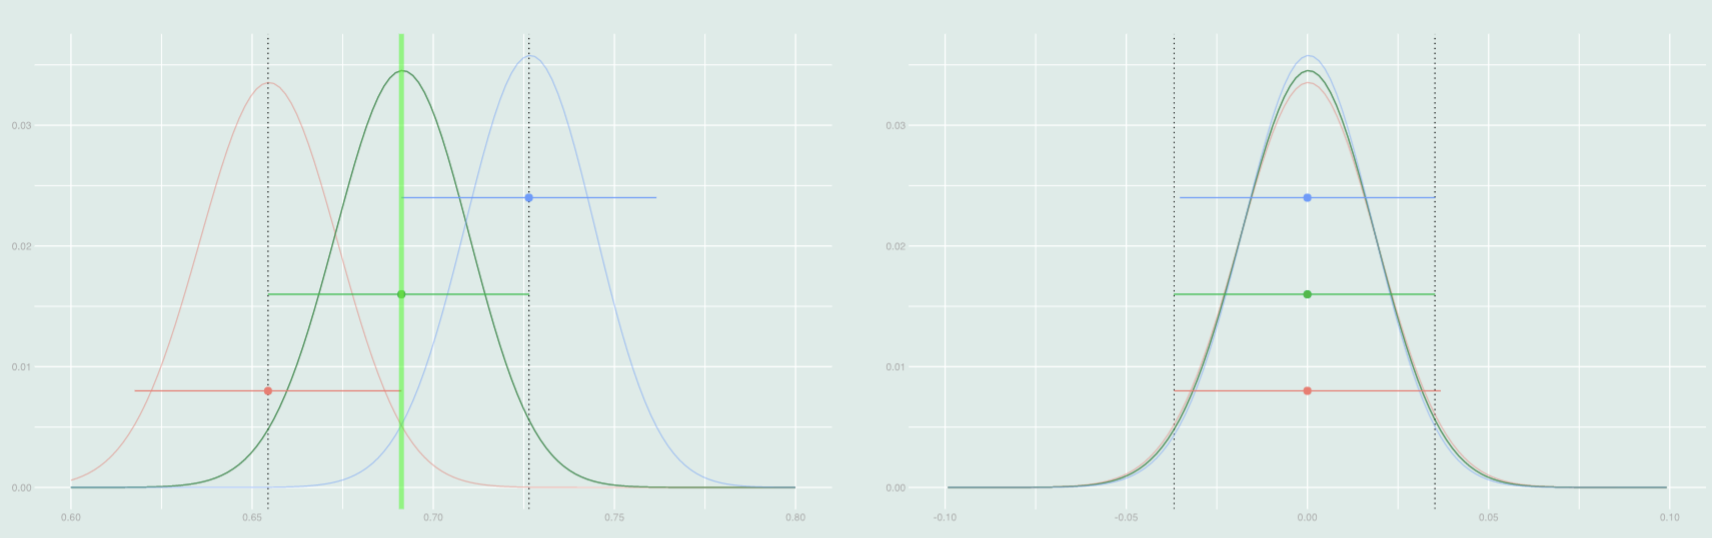
\includegraphics[width=0.7\textwidth]{figs/BinomialDistribution.png}\end{center}	
	The Binomial distribution is \textit{continuous} as a function of $p$, so when $p$ cahgnes little, the distribution changes little. That is to say that if we are not far off in the proportion, the estimated and actual sampling distributions are similar. The relevant difference (after centering) is even smaller because the way the binomial changes is mostly location. \par 
	This can be thought of a sort of ``confidence interval'' for our estimate of the sampling distribution. 95\% of the time, we will get an estimate somewhere between the {\color{red}{red}} and {\color{blue}{blue}} ones. As a result, a width of our interval estimate somewhere between the red and blue widths. 
\end{eg}
\begin{eg}{The Bootstrap Interpretation}
	Let's revisit our distribution: \[\text{Binomial}(n,p)/n.\]	This sample distribution indicates the proportion of $1$'s if we poll a sample of $n$ object among whom the proportion of $1$'s is exactly $\bar{Y}=p$. This means that we can get a draw from our estimated sampling distribution by running a ``poll'' of the objects in our sample: rolling a $n$-sided die $n$ times, calling up the corresponding object in our sample, and counting up the $1$'s we observe.  
\end{eg}
\begin{lstlisting}[title=Boostraping Sample, language=r]
bootstrap.samples = array(dim=10000)
for (rr in 1:10000) {
	Y.boot = Y[sample(1:n, n, replace=TRUE] # Boostraping
	bootstrap.samples[rr] = sum(Y.boot)/n
}
\end{lstlisting}


\begin{rmk}[Bootstrap Sampling]
	The usual way of sampling is to use a sample to approximate the population. Since one sample can only generate one estimate, we need many samples. However, we cannot do this in reality. Instead, we only have one sample, so we will use bootstrapping. In that way, we resample the sample multiple times to general different estimates. Using the resampling distribution, we can eventually approximate the population. 
\end{rmk}
\begin{df}{Normal Distribution}
	The \textit{normal distribution} is a function of two parameters: its mean and its standard deviation: \[p_{\mu,\sigma}(x)=\dfrac{1}{\sqrt{2\pi}\sigma}e^{-\frac{(x-\mu)^2}{2\sigma^2}}\]
\end{df}
\begin{thm}{Central Limit Theorem}
	The sampling distribution and the bootstrap sampling distribution is approximately normal, and this is a consequence of the Central Limit Theorem. 
\end{thm}

\subsection{Probability Review}
\begin{thm}{Properties of Expectations}
	\begin{description}
		\item[Linearity of Expectation] Suppose $Y,Z$ are random variables and $a,b\in\R$. Then \[\E(aY+bZ)= \E(aY)+\E(bZ)=a\E(Y)+b\E(Z).\] 
     	\item[Multiplication Rules] Suppose $Y,Z$ are independent ($\independ$) random variables, then \[\E(Y\cdot Z)=\E(Y)\cdot\E(Z).\]
	\end{description}
\end{thm}
\begin{rmk}
	Without special notice, we assume random variables are independent in this course.	
\end{rmk}
\begin{thm}{Variacne Decomposition}
	If $Y\independ Z$, then $\Var(Y+Z)=\Var(Y)+\Var(Z).$	
\end{thm}
\begin{prf}
	Notice that  \begin{align*}\Var(Y+Z)&=\E[(Y+Z)^2]- \E(Y+Z)^2\\&=\E(Y^2+Z^2+2YZ)-[\E(Y)+\E(Z)]^2 \\
    &=\E(Y^2)+\E(Z^2)+2\E(YZ)-\E(Y)^2-\E(Z)^2-2\E(Y)\E(Z)&[\text{Linearity}]\\&=(\E(Y^2)-\E(Y)^2)+(\E(Z^2)-\E(Z)^2)+2\E(YZ)-2\E(YZ)&[\text{Independence}]\\&=\Var(Y)+\Var(Z).\end{align*}
\end{prf}
\begin{thm}{Binomial Expection and Variance}
	If $Y\sim\text{Binomial}(n,p)$, then \[\E\qty(\bar{Y})= \E\qty[\dfrac{1}{n}\sum_{i=1}^n(Y_i)]=p\] and \[\Var\qty(\bar{Y})=\dfrac{p(1-p)}{n}.\] The proof of these two quantities are omitted. 
\end{thm}
\begin{df}{Conditional Expectation}
    The \textit{conditional expectation} is $\E[Y\mid X=x]$, namely the expected value of $Y$ given that $X=x$.
\end{df}
\begin{thm}{Properties of Conditional Expectation}
	\begin{description}
		\item[Law of Iterated Expectations] for any random variables $X$ and $Y$, we have \[\E(Y)=\E\qty{\E(Y\mid X)}.\]
		\item[Irrelevance of Independent Conditioning Variables] When $Z\independ X$ and $Y$, we have \[\E(Y\mid X,Z)=\E(Y\mid X).\] In other words, if $Z$ is unrelated to $X$ and $Y$, holding it constant does not affect the relationship between $X$ and $Y$.
	\end{description}
\end{thm}
\end{document}